%\documentclass[a4paper, english,10pt]{article}
%\documentclass[english,10pt, oneside, draft, a4paper]{report}
\documentclass[english,10pt, oneside, a4paper]{article}
%\usepackage[b5paper, layout=b5paper, textwidth=12cm, twoside,bindingoffset=1cm,outer=2cm,inner=2cm,includefoot,bmargin=3cm]{geometry}
\usepackage[a4paper, layout=a4paper, textwidth=12cm, bindingoffset=1cm,outer=2cm,inner=2cm,includefoot,bmargin=3cm]{geometry}
\usepackage[english]{babel}
\usepackage[utf8]{inputenc}
\usepackage[T1]{fontenc}
\usepackage{float}
\usepackage{subfig}
\usepackage{multirow}
\usepackage{tabularx}
\usepackage{perpage} % For å få fotnotenummerering til å starte på nytt for hver side
\usepackage{graphicx}
\usepackage{subfig}
\graphicspath{{../../grafikk/}}

\usepackage{usecases}
\usepackage{varioref}

\linespread{1.5}

% ##### Defines NoIndent a way to have text that isn't a part of a list and 
% doesn't indent. The text will also survive pagebreaks. 
\newbox\totalbox
\newbox\partialbox
\newdimen\partialboxdim

\newenvironment{nibox}
  {\par\vskip-6pt\setbox\totalbox=\vbox\bgroup}
  {\egroup\splitnibox}

\def\splitnibox{%
  \ifvoid\totalbox\par
  \else\continuesplitting\fi}

\def\continuesplitting{\null% In case this starts a new page
  \dimen255=\dimexpr\pagegoal-\pagetotal-\pageshrink-6pt\relax
  \ifdim\ht\totalbox<\dimen255
    \setbox\partialbox=\box\totalbox
    \unvbox\partialbox
  \else
    \setbox\partialbox=\vsplit\totalbox to\dimen255
    \unvbox\partialbox\eject
  \fi
  \splitnibox}

\newcommand\NoIndent[1]{\begin{nibox}#1\end{nibox}}
% End of the new command.

\begin{document}
\clearpage
\title{System Requirements Document}
\author{Magnus Bae and Magnus Krane\\ NTNU}
\date{December 2013}
%\maketitle

\makeatletter
\renewcommand{\l@section}{\@dottedtocline{1}{1.5em}{2.6em}}
\renewcommand{\l@subsection}{\@dottedtocline{2}{4.0em}{3.6em}}
\renewcommand{\l@subsubsection}{\@dottedtocline{3}{7.4em}{4.5em}}
\makeatother
\renewcommand{\thesection}{D.\arabic{section}}%Change to correct appendix nr

\setcounter{tocdepth}{5}
\setcounter{secnumdepth}{5}


\setcounter{page}{55}
\clearpage
\renewcommand\contentsname{Table of Contents}
\tableofcontents

% !TEX root=../thesis.tex

\chapter{Introduction}

In this report we aim to design a software architecture for a driver information
system\footnote{Also known as In Vehicle Information System, IVIS}
that is to be prototyped and installed in a formula student race car. We will
also discuss the state of the art, technological alternatives and introduce
background information pertaining to the domain and use-cases.

To design this architecture we have undertaken a significant literature study
of both architectural design patterns and driver/operator information systems.
We have looked at what a typical driver information system does, how it does
it, and what the state of the art is. Other fields employing information 
systems to provide vehicle operators with real-time information have also been
studied.

This research effort is made to serve as a foundation to build a prototype
driver information system in collaboration with Revolve NTNU (Revolve), a 
student organization  created by students at the Norwegian University of 
Science and Technology.
The the collaboration with Revolve will serve as a testing ground for our 
design and allow us to test its feasibility in the
context of motorsport.

For the last three years Revolve has been hard at work building formula style race
cars to participate in events of the international motor sport competition series
``Formula Student'' (FS). The competitions are arranged by the Institution of Mechanical Engineers. In the competitions teams of students compete against each other
with small formula-style cars they have designed and built from scratch. There are
disciplines that involves racing the cars as well as disciplines in business,
design, and cost. The combined score from these events decide the official
results, but there are also prices awarded for excellence in different fields

Motorsport has for many years been a testbed for car manufacturers and a lot of
technology that we today take for granted has come to fruition through motorsport. However
ordinary cars have seen larger leaps in technology with regards to information
consumption than cars built for motor racing. For some years some high-end cars
have even been equipped with heads-up displays (HUD) that allows the driver to 
keep focus on the road instead of looking down at the instruments \cite{wiki:hud},
and it is becoming more and more common.

Despite great developments in automobile technology over the past 50 years little
has changed in the way that motorsport drivers receives information during an
event. There are displays, gauges, and other visual indicators\footnotemark[1]
, in addition to radio-communication \cite{wiki:formula_radio} if that is allowed in the competition. The technology under the hood
has become much more advanced, but the amount of information you can
convey to the driver still seems to be very limited; the pace is just too high
to be able to keep moving focus from the road (see appendix \vref{interview:bakkom}).

Driver information systems in the context of motorsport is a field neglected by
science (see \vref{background:rel_reasearch}). There has been done some
research around driver information systems in commercial vehicles and normal 
passenger cars, most of which involve studies of heads-up display technology or
use.

This is therefore a field where we are threading into new territory. 
Requirements are hard to elicit up front, and we don't know
from the start what is a good design for such a system. It is quite possible
that requirement changes can come from opportunities enabled by 
creating a new system that can potentially deliver more information to the
driver with faster response times (from the driver) and less distractions. 
This means that any system developed must be flexible enough to allow for easy 
experimenting with configuration
alternatives and have a high-level support for requirements evolution.

The question we want to address in this report is as follows; How can we
enable the development of a state of the art computerized driver information system
by creating a software architecture that is flexible enough to allow easy
experimenting and customization?

The rest of this document is divided into several parts. In the background chapter we will
discuss the collaboration with Revolve NTNU and present the Formula Student
competition. We also present relevant electronic principles and knowledge and discuss the current
state of research with a focus on automotive information systems. Chapter \vref{chapter:method}
introduces the methods we've applied in our work, while
the following chapter (\vref{chapter:results}) shows the findings of our research.
Then we discuss our findings and try to put them in perspective in chapter \vref{chapter:discussion}, before we move
onto the conclusion and discussing recommendations and possibilities for
further work in chapter \vref{chapter:conclusion}.
The appendices contain development artifacts created during the design process
and details the results and the information they build upon, as well as an interview with a driver from last years Revolve-team. 


\footnotetext{
	Although extensive research has been performed scientific, 
	findings are rare. Cottle et al.. \cite{wirelessDashboard} discusses implementing a 
	wireless ``dashboard'' (controls and instruments on a steering wheel). 
	Although lacking scientific base the statement should hold; this 
	assumption is made stronger by analyzing motorsport on TV and for 
	pictures of race cars' interiors.
}


% !TEX root=../document.tex

\section{Use Cases}

	%Sometimes it is a good idea to put domain objects in \texttt{}
	%The template and the descriptions are based on the book Applying UML and Patterns: 
	%An Introduction to Object-Oriented Analysis and Design and Iterative Development
	%(3rd Edition) by Craig Larman.
	% \begin{usecase}

	% 	\addtitle{Use Case 0}{Template} 
	% 	\addfield{Scope:}{System-wide} %Scope: the system under design
	% 	\addfield{Level:}{User-goal} %Level: "user-goal" or "subfunction"
	% 	\addfield{Primary Actor:}{End-User} %Primary Actor: Calls on the system to deliver its services.
	% 	\additemizedfield{Stakeholders and Interests:}{ %Stakeholders and Interests: Who cares about this use case and what do they want?
	% 		\item Stakeholder 1 name: his interests
	% 		\item Stakeholder 2 name: his interests
	% 	}
	% 	\addfield{Preconditions:}{} %Preconditions: What must be true on start and worth telling the reader?
		
	% 	%when multiple
	% 	%\additemizedfield{Preconditions:}{} 

	% 	\addfield{Postconditions:}{}%Postconditions: What must be true on successful completion and worth telling the reader
		
	% 	%when multiple
	% 	%\additemizedfield{Preconditions:}{}

	% 	\addscenario{Main Success Scenario:}{ %Main Success Scenario: A typical, unconditional happy path scenario of success.
	% 		\item The first action
	% 		\item The second action
	% 	}
	% 	\addscenario{Extensions:}{ %Extensions: Alternate scenarios of success or failure.
	% 		\item[2.a] Invalid login data:
	% 			\begin{enumerate}
	% 			\item[1.] System shows failure message
	% 			\item[2.] User returns to step 1
	% 			\end{enumerate}
	% 		\item[5.a] Invalid subsriber data:
	% 			\begin{enumerate}
	% 			\item[1.] System shows failure message
	% 			\item[2.] User returns to step 2 and corrects the errors
	% 			\end{enumerate}
	% 	}

	% 	\additemizedfield{Special Requirements:}{ %Special Requirements: Related non-functional requirements.
	% 		\item first applicable non-functional requirement
	% 		\item second applicable non-functional requirement
	% 	}
	% 	\addscenario{Technology and Data Variations List:}{ %Technology and Data Variations List: Varying I/O methods and data formats.
	% 		\item[1a.] Alternative first action with other technology
	% 	}
	% 	\addfield{Frequency of Occurrence:}{}%Frequency of Occurrence: Influences investigation, testing and timing of implementation.

	% 	%Miscellaneous: Such as open issues/questions
	% 	%\addfield{Open Issues:}{}
	% \end{usecase}

	% \begin{usecase}
	% 	\addtitle{Use Case 0}{Empty Template} 
	% 	\addfield{Scope:}{System-wide} 
	% 	\addfield{Level:}{User-goal} 
	% 	\addfield{Primary Actor:}{End-User} 
	% 	\additemizedfield{Stakeholders and Interests:}{
	% 		\item Stakeholder 1 name: his interests
	% 		\item Stakeholder 2 name: his interests
	% 	}
	% 	\addfield{Preconditions:}{} 
	% 	\addfield{Postconditions:}{}
	% 	\addscenario{Main Success Scenario:}{ 
	% 		\item The first action
	% 		\item The second action
	% 	}
	% 	\addscenario{Extensions:}{ 
	% 		\item[2.a] Invalid login data:
	% 			\begin{enumerate}
	% 			\item[1.] System shows failure message
	% 			\item[2.] User returns to step 1
	% 			\end{enumerate}
	% 		\item[5.a] Invalid subsriber data:
	% 			\begin{enumerate}
	% 			\item[1.] System shows failure message
	% 			\item[2.] User returns to step 2 and corrects the errors
	% 			\end{enumerate}
	% 	}

	% 	\additemizedfield{Special Requirements:}{ 
	% 		\item first applicable non-functional requirement
	% 		\item second applicable non-functional requirement
	% 	}
	% 	\addscenario{Technology and Data Variations List:}{ 
	% 		\item[1a.] Alternative first action with other technology
	% 	}
	% 	\addfield{Frequency of Occurrence:}{}
	% \end{usecase}

	\begin{usecase}
		\addtitle{\label{uc_formatconf}Use Case UC\ref{uc_formatconf}}{Configure message format} 
		\addfield{Scope:}{Configuration system} 

		\addfield{Primary Actor:}{Developer or system implementer} 
		\additemizedfield{Stakeholders and Interests:}{
			\item System implementer: Wants to be able to move system into another
			vehicle without having to recompile source code and re-program the system.
			\item System developer (developer): Wants to be able to easily adjust for
			changing message formats or if a sensor or message should need a special
			message format, also would like to avoid to have to recompile and program in
			new firmware if message format changes.
			\item Revolve NTNU: Wants to have the possibility to change the message
			format without having to use big amounts of time to adjust the Driver Information
			System (DIS).
		}
		\addfield{Preconditions:}{} 
		\addfield{Postconditions:}{A message format configuration is recorded by the
		system
		}
		\addscenario{Main Success Scenario:}{ 
			\item Actor starts to create a new message format.
			\item Actor defines the standard message frame format.
			\item Actor defines what is accepted as a valid message.
			\item Actor defines which part of the message contains the sensor identification
			or message detail.
			\item Actor defines which part of the message which contains the raw data from the sensor.
			\item Actor asks the system to record configuration.
			\item \label{uc_formatconf:save}System acknowledges that configuration has
			been recorded.
			\NoIndent{\textit{These steps can be repeated to create multiple message
			formats if needed}}
		}
		\addscenario{Extensions:}{ 
			\item[\ref{uc_formatconf:save}.a] Error recording configuration:
				\begin{enumerate}
					\item[1.] System displays an error message explaining the error
					\item[2.] Actor can retry step, ie. save to another location or try again (in
					the case of removable or network media)
				\end{enumerate}
		}
		\additemizedfield{Special Requirements:}{ 
			\item The message format should be general enough to accept frame formats
			for different types of communication networks/protocols.
		}
	\end{usecase}
	\clearpage



	\begin{usecase}
		\addtitle{\label{uc_sensconf}Use Case UC\ref{uc_sensconf}}{Configure sensors} 
		\addfield{Scope:}{Configuration system} 

		\addfield{Primary Actor:}{Developer, system implementer or system owner (future)} 
		\additemizedfield{Stakeholders and Interests:}{
			\item Future owner of system: Wants to be able to adapt and change 
			the configuration of sensors (broken sensor, changing sensor, etc.)
			\item System implementer: Wants to be able to choose which sensors 
			are to be used for data collection and ignore others. To easily be 
			able to turn sensors on and off.
			\item System developer (developer): Wants to experiment with 
			sensor usage and to easily choose which sensors are to be 
			included, swap between different sensor configurations and choose 
			different setups for testing and development. 
			\item Revolve NTNU: Wants configuration to be a process that can 
			be done with minimal interfacing on the car so that other 
			processes will not be disturbed. 
			\item Driver (competition): Wants a setup of sensors that are 
			relevant for the competition at hand and can help increasing 
			performance
			\item Driver (training): Wants a setup of sensors that provide the 
			information wanted during training and assist in assessing own 
			abilities and possible improvement areas.
			\item Driver (rental): Wants to get information that can show 
			performance and make it easy to see progress between laps and 
			learn where there is room for improvement.
		}
		\addfield{Preconditions:}{Requires one or more configured message formats
		(see UC\ref{uc_formatconf})
		} 
		\additemizedfield{Postconditions:}{
			\item A sensor configuration is created and recorded by
			the system.
			\item Each recorded sensor has a valid input-output mapping
		}
		\addscenario{Main Success Scenario:}{ 
			\item Actor starts to create a new sensor setup
			\item \label{uc_sensconf:chooseMessageFormat}Actor selects default message
			format.
			\item \label{uc_sensconf:start}Actor enters sensor identifier string.
			\item \label{uc_sensconf:messformat}System automatically chooses the default message format and
			displays this. 
			\item Actor enters the sensors expected message ID or address
			\item Actor enters the sensors expected input unit
			\item Actor enters the output unit (transformation of input value)
			\item Actor enters the sensors linear calibration algorithm 
			\item \label{uc_sensconf:value_range}Actor selects or enters the valid value-range for the sensor. 
			\item Actor gives priority to sensor display.
			\item Actor may choose to add aggregation rule.
			\item Actor may choose to add add trigger-event for sensor (can be triggered from
			other sensors)
			\item \label{uc_sensconf:stop}System records the sensor information and shows the information from all registered sensors. 
			\NoIndent{\textit{Actor repeats step \ref{uc_sensconf:start} to \ref{uc_sensconf:stop} until done}}
			\item \label{uc_sensconf:save}Actor asks the system to record the sensor configuration and the system acknowledges. 
		}
		\addscenario{Extensions:}{ 
			\item[\ref{uc_sensconf:messformat}.a] Actor wishes to use non-default
			format:
				\begin{enumerate}
					\item[1.] Actor chooses another predefined message format.
					\item[2.] Actor continues with the next step.
				\end{enumerate}
			\item[\ref{uc_sensconf:messformat}.b] Actor wishes to use a yet undefined
			message format:
				\begin{enumerate}
					\item[1.] Actor chooses to define a new message format for use with
					this sensor configuration.
					\item[2.] Actor follows the steps outlined in UC\ref{uc_formatconf}.
					\item[3.] Upon recording the message format the system 
					returns to  step \ref{uc_sensconf:messformat}
					with the new format selected for the active sensor.
					\item[4.] Actor continues with the next step.
				\end{enumerate}
			%end of message format deviations (extensions).

			\item[\ref{uc_sensconf:value_range}.a] Sensor with multiple acceptable output units:
				\begin{enumerate}
					\item[1.] Actor can choose to add a unit to the value mapping that can
					be utilized by the display mapping (see UC\ref{uc_dispconf}).
				\end{enumerate}
			\item[\ref{uc_sensconf:save}.a] Error recording configuration:
				\begin{enumerate}
					\item[1.] System displays an error message explaining the error
					\item[2.] Actor can retry, eg. save to another location or try again (in
					the case of removable or network media)
				\end{enumerate}
		}
		\additemizedfield{Special Requirements:}{ 
			\item A sensor can also be a standalone subsystem communicating status of
			one or more sensors or actively controlled units.
			\item A sensor configuration must support having sensors with different 
			formats.
			\item In the case a sensor or subsystem sends messages using different
			formats the system shall support having multiple instances of a sensor with
			varying frame formats.
		}
		\addscenario{Technology and Data Variations List:}{ 
			\item[A] If there is a duplex communication link between the car and radio and support team it should also be possible to receive messages.
		}
	\end{usecase}
	\clearpage



	\begin{usecase}
		\addtitle{\label{uc_dispconf}Use Case UC\ref{uc_dispconf}}{Configure display} 
		\addfield{Scope:}{Configuration system} 

		\addfield{Primary Actor:}{Driver, Developer, system implementer or system owner (future)} 
		\additemizedfield{Stakeholders and Interests:}{
			\item Future owner of system: Wants to be able to adapt and change 
			the display of information from sensors (customer demand, new ideas)
			\item System implementer: Wants to be able to adapt and change the display of information from different sensors based on preferences or
			requests.
			\item System developer (developer): Wants to experiment with 
			sensor display models, easily try out various configurations and have a quick deploy-time for a new configuration. 
			\item Revolve NTNU: Wants configuration to be a process that can 
			be done with minimal interfacing on the car so that other 
			processes will not be disturbed. Also wants to be able to vary the display for various circumstances and to be able to experiment with what works best to get the best performance out of the drivers. 
			\item Driver (competition): Wants a display configuration that is tailored
			to the event and displays the most relevant information.
			\item Driver (training): Wants a display that is tailored for training and
			enables the driver to better assess own performance and areas of
			improvement.
			\item Driver (rental): Wants to get information that can show 
			performance and make it easy to see progress between laps and 
			learn where there is room for improvement.
		}
		\addfield{Preconditions:}{There already exists one or more sensor configurations profiles (See UC\ref{uc_sensconf})} 
		\addfield{Postconditions:}{A display configuration is created and recorded by
		the system.}
		\addscenario{Main Success Scenario:}{ 
			\item Actor creates a new display configuration.
			\item Actor loads a sensor configuration.
			\item \label{uc_dispconf:start}Actor chooses a sensor.
			\item System presents available representations for that sensor
			\item Actor places the sensor.
			\item \label{uc_dispconf:stop}Actor configures the sensor display size.
			\NoIndent{\textit{Actor repeats step \ref{uc_dispconf:start} to \ref{uc_dispconf:stop} until done.}}
			\item \label{uc_dispconf:save}Actor chooses to record the display configuration and the system acknowledges.
		}
		\addscenario{Extensions:}{ 
			\item[\ref{uc_dispconf:save}.a] Error saving file:
				\begin{enumerate}
					\item[1.] The system displays an error message explaining the error
					\item[2.] The actor can retry the step, for instance save to another location or try again (in
					the case of removable or network media)
				\end{enumerate}
		}

		\additemizedfield{Special Requirements:}{ 
			\item first applicable non-functional requirement
			\item second applicable non-functional requirement
		}
		\addscenario{Technology and Data Variations List:}{ 
			\item[1.a] Alternative first action with other technology
		}
	\end{usecase}
	\clearpage



	\begin{usecase}
		\addtitle{\label{UC:Configuration-upload}Use Case UC\ref{UC:Configuration-upload}}{Upload configuration} 
		\addfield{Scope:}{System-wide} 

		\addfield{Primary Actor:}{Driver, Developer, system implementer or system owner (future)} 
		\additemizedfield{Stakeholders and Interests:}{
			\item Future owner of system: Wants to be able to adapt and change 
			the display of information from sensors (customer demand, new ideas). Wants uploading of a new configuration to be a quick,
			easy and robust process.
			\item System implementer: Wants uploading of a new configuration to be a quick,
			easy and robust process.
			\item System developer (developer): Wants to experiment with 
			sensor usage and to easily choose which sensors are to be 
			included, swap between different sensor configurations and choose 
			different setups for testing and development. 
			\item Revolve NTNU: Wants configuration to be a process that can 
			be done with minimal interfacing on the car so that other 
			processes will not be disturbed. 
			\item Driver (competition): Wants changing of setups to be a quick process.
			\item Driver (training): Wants changing of setups to be a quick process,
			also wants to try different setups to find what works best.
			\item Driver (rental): Wants configuration to be a transparent process, and
			the possibility to select the setup of his or hers choosing. 
		}
		\addfield{Preconditions:}{There already exists one or more display configuration profile (see UC\ref{uc_dispconf})} 
		\addfield{Postconditions:}{A display- and sensor configuration is uploaded
		to the driver information system.}
		\addscenario{Main Success Scenario:}{ 
			\item Actor opens a display configuration profile.
			\item \label{uc_upload_powerup}Actor turns on the driver information system (DIS).
			\item \label{uc_upload_connection}Actor creates a connection between the configuration system and
			the DIS. 
			\item Actor initiates an upload of the configuration to the DIS and the
			system displays progress during the process.
			\item \label{uc_upload_complete}System completes the upload and displays a success message.
			\item DIS loads the configuration profile and is ready for use.
		}
		\addscenario{Extensions:}{ 
			\item[\ref{uc_upload_powerup}.a] DIS lacks power:
				\begin{enumerate}
					\item[1.] DIS does not indicate power or activity
					\item[2.] Actor gives DIS external power and continues with next step.
				\end{enumerate}
			\item[\ref{uc_upload_connection}.a] No connection established:
				\begin{enumerate}
					\item[1.] System shows failure message
					\item[2.] Actor can choose to abort or retry.
				\end{enumerate}
			\item[\ref{uc_upload_complete}.a] Upload fails:
				\begin{enumerate}
					\item[1.] System shows failure message with explanation of error.
					\item[2.] Actor can choose to retry or try to take action to rectify problem.
				\end{enumerate}
		}
		\addscenario{Technology and Data Variations List:}{ 
			\item[\ref{uc_upload_connection}.a] Connection can be made using an applicable
			interface for the technology utilized, it may be wireless or wired.
			There is no predefined protocol. 
		}
	\end{usecase}
	\clearpage


\begin{usecase}
		\addtitle{\label{uc_sendMessage}Use Case UC\ref{uc_sendMessage}}{Send message to driver} 
		\addfield{Scope:}{Display system} 
		\addfield{Primary Actor:}{Support team member or system owner} 
		\additemizedfield{Stakeholders and Interests:}{
			\item Revolve NTNU: Wants ways to effectively communicate information during
			training (two-way communication not allowed during competitions).
			\item Driver (competition): Wants to be able to receive textual messages in
			case radio-communication isn't feasible. 
			\item Driver (training): Wants to be able to receive messages or alerts from
			support team.
			\item Driver (rental): Wants to be able to receive messages or alerts from
			system owner or other involved parties.
		}
		\additemizedfield{Preconditions:}{
			\item DIS is configured to receive messages.
			\item DIS is running and communicating.
			\item DIS has a way of establishing a wireless communication with the
			external system. 
		} 
		\addfield{Postconditions:}{DIS receives and displays a received message.}
		\addscenario{Main Success Scenario:}{ 
			\item Actor tells system to create a new message.
			\item \label{uc_sendMessage:create}(Support) System asks user to enter message and priority.
			\item Actor enters message and sends it.
			\item \label{uc_sendMessage:wireless}System sends message over wireless medium.
			\item \label{uc_sendMessage:disReceive}DIS receives message.
			\item \label{uc_sendMessage:evalPri}DIS evaluates priority of message.
			\item DIS displays message in a timely manner based on priority.
			\item \label{uc_sendMessage:sendAck}DIS sends message back acknowledging message has been displayed.
		}
		\addscenario{Extensions:}{
			\item[\ref{uc_sendMessage:disReceive}.a] DIS does not receive message: See
			extension \ref{uc_sendMessage:sendAck}.

			\item[\ref{uc_sendMessage:sendAck}.a] \label{uc_sendMessage:extResend}Support system does not receive
			acknowledgment from DIS within 10 seconds:
				\begin{enumerate}{
					\item[1.] System resends message.
					\item[2.] DIS receives message.
					\item[3.a] DIS has received first message, but awaiting display due to
					priority and therefore discards message
					\item[3.b] DIS has not received first message, returns to step \ref{uc_sendMessage:evalPri}
				}
				\end{enumerate}
		}
		\addscenario{Technology and Data Variations List:}{ 
			\item[\ref{uc_sendMessage:create}.a] If vehicle has positioning actor might
			also select position for message to be displayed, for instance avoiding
			displaying messages in corners. This requires tracking vehicle in either DIS
			or support system. 
			\item[\ref{uc_sendMessage:wireless}.a] Depending on technology chosen DIS
			should be able to receive messages from vehicle sub-systems and/or a
			dedicated communications channel. 
		}
	\end{usecase}
	\clearpage


	\begin{usecase}
		\addtitle{\label{UC:Information-display}Use Case UC\ref{UC:Information-display}}{Display real-time information} 
		\addfield{Scope:}{Display system} 
		\addfield{Primary Actor:}{DIS} 
		\additemizedfield{Stakeholders and Interests:}{
			\item Revolve NTNU: Wants the system to be effective and correct to give
			advantages during training and competitions
			\item Driver (competition): Wants to be able to get a hold of essential
			and/or critical information without losing focus of the driving.
			\item Driver (training): Wants to be able to easily get information about
			own performance and possible areas of improvement. Would also like to get
			alerted when receiving messages (see UC\ref{uc_sendMessage}) from support team and monitor vehicle status.
			\item Driver (rental): Wants to be able to easily get information about
			own performance and possible areas of improvement.
		}
		\additemizedfield{Preconditions:}{
			\item DIS is configured for the cars sensor load-out.
			\item DIS is configured with the correct display layout.
			\item DIS is powered up (operational), awaiting data.
			\item Driver is seated in the vehicle.
			\item Vehicle is powered up and the sensor network is active.
		} 
		\addfield{Postconditions:}{DIS works without problems during the driving.}
		\addscenario{Main Success Scenario:}{ 
			\item Driver adjusts the position of the DIS if applicable.
			\item \label{uc:sensor_read_start}DIS reads sensor information at given intervals or when received
			through the sensor network.
			\item DIS processes the raw sensor data and transforms it into real
			world data using the settings in the configuration profile (see UC\ref{uc_sensconf})
			\item DIS evaluates importance of information compared to sensed activity
			and priority rules.
			\item \label{uc4:sound_also}\label{uc:sensor_read_stop}DIS transforms the calibrated sensor data
			into graphical output.
			\NoIndent{\textit{System repeats step \ref{uc:sensor_read_start} to
			\ref{uc:sensor_read_stop} until powered down or it stops receiving data}}
		}
		\additemizedfield{Special Requirements:}{ 
			\item DIS automatically loads the last configuration.
			\item DIS does not distract the driver.
			\item DIS should deliver information from sensors with less than 200ms
			delay.
			\item DIS should not process information from sensors not configured.
			\item DIS shall not obstruct the drivers entry or exit from the vehicle.
		}
		\addscenario{Technology and Data Variations List:}{ 
			\item[\ref{uc4:sound_also}.a] DIS might also use sounds if technology allows it and found as an appropriate means of giving information. 
		}
	\end{usecase}
	\clearpage


\subsection{Additional requirements}
The system shall:
	\begin{itemize}
		\item deliver information to the driver with less than 200 ms delay 90\% of the time.
		\item not negatively affect the drivers performance.
		\item not obstruct the drivers entry or exit from the vehicle.
	\end{itemize}

% !TEX root=../document.tex

\section{Conceptual model}

\subsection{System sequence diagrams}

\subsubsection{SSD - Configure Message Format}
\begin{figure}[!htbp]
  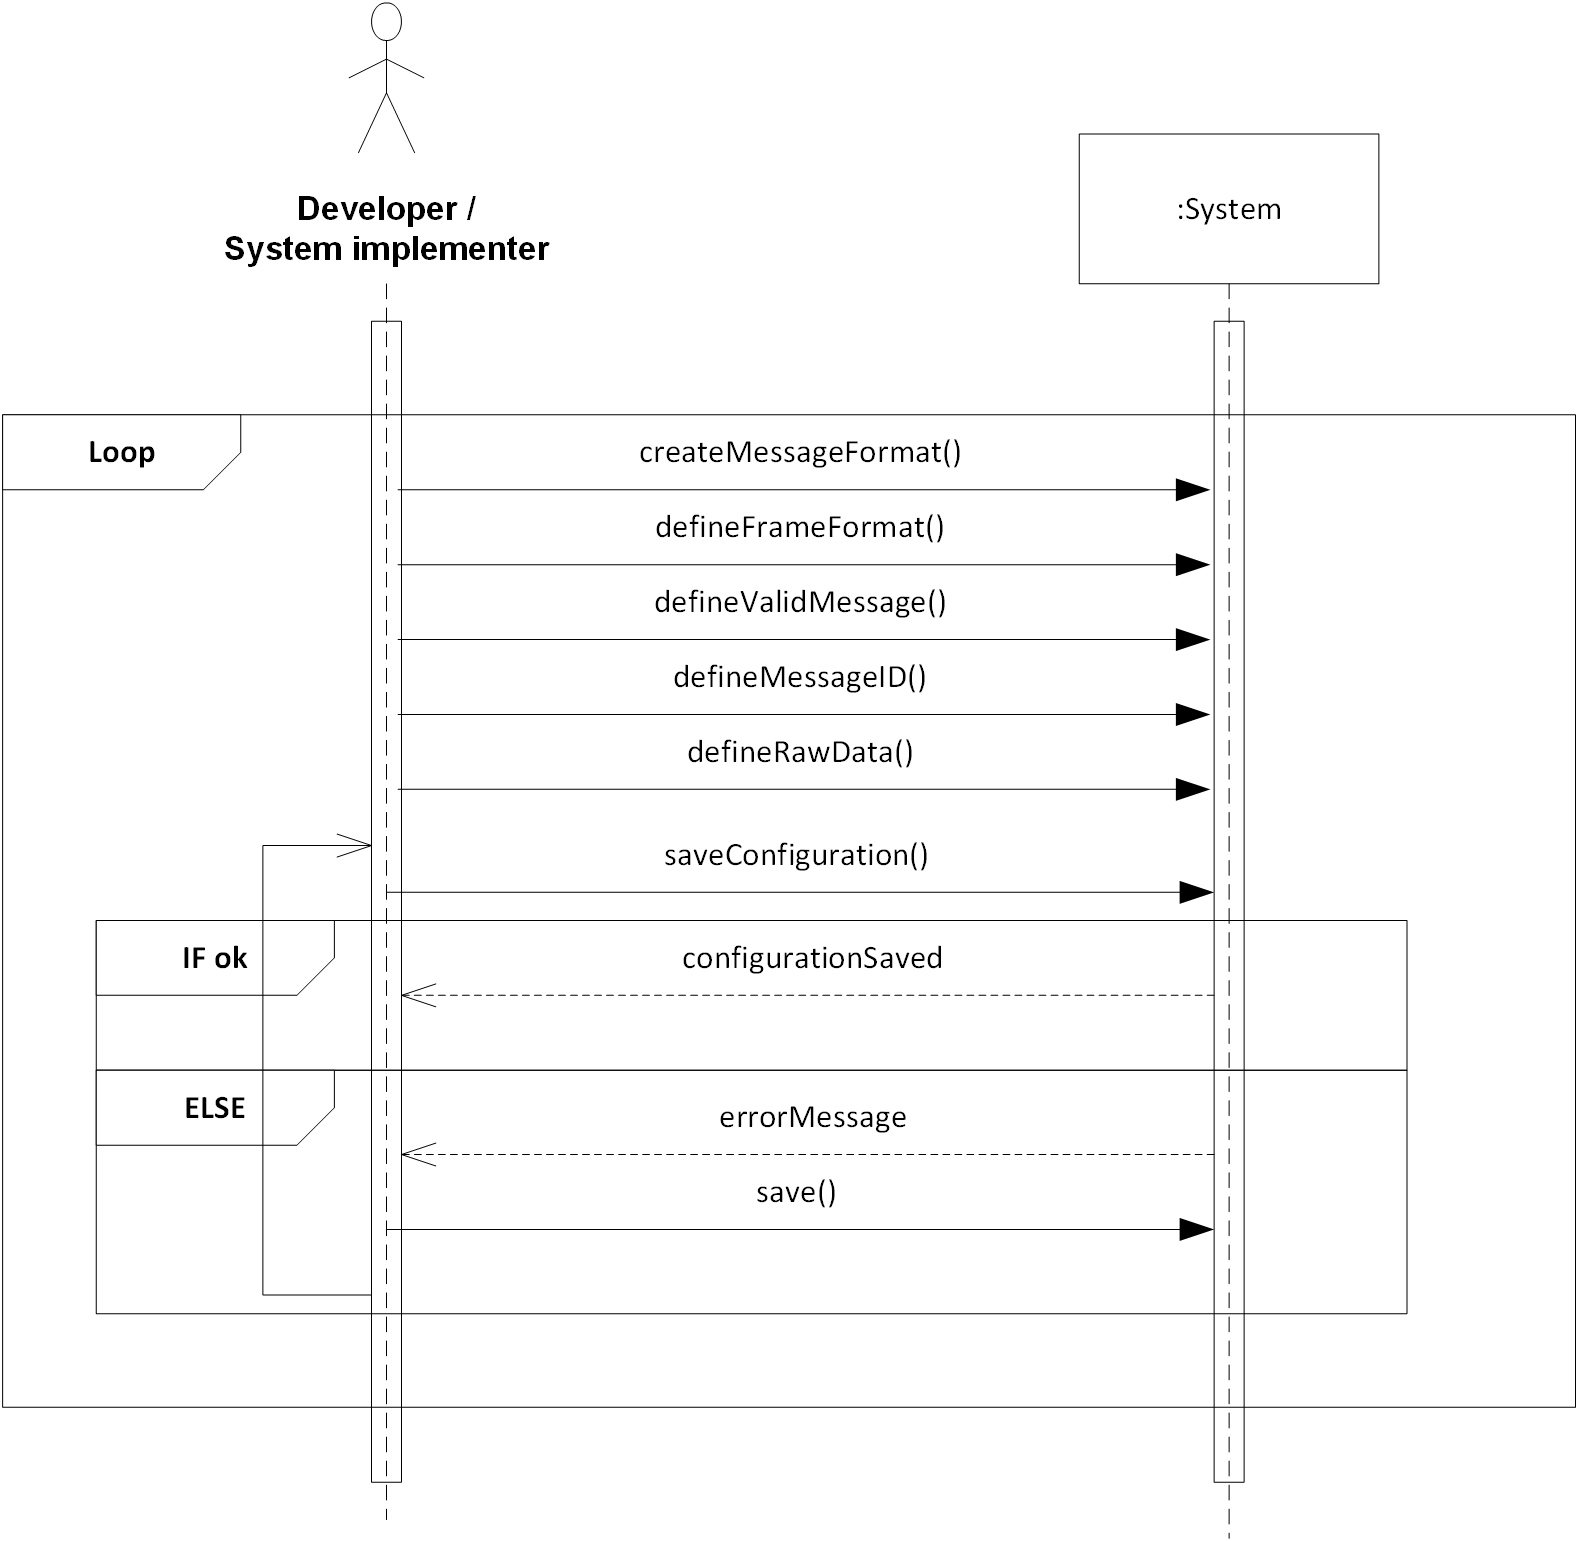
\includegraphics[width=\textwidth]{SSD-Configure-Message-Format.png}
  \caption{SSD for UC\vref{uc_formatconf}}
  \label{fig:SSD-Configure-Message-Format}
\end{figure}
\clearpage

\subsubsection{SSD - Configure Sensors}
\begin{figure}[!htbp]
  \ContinuedFloat
  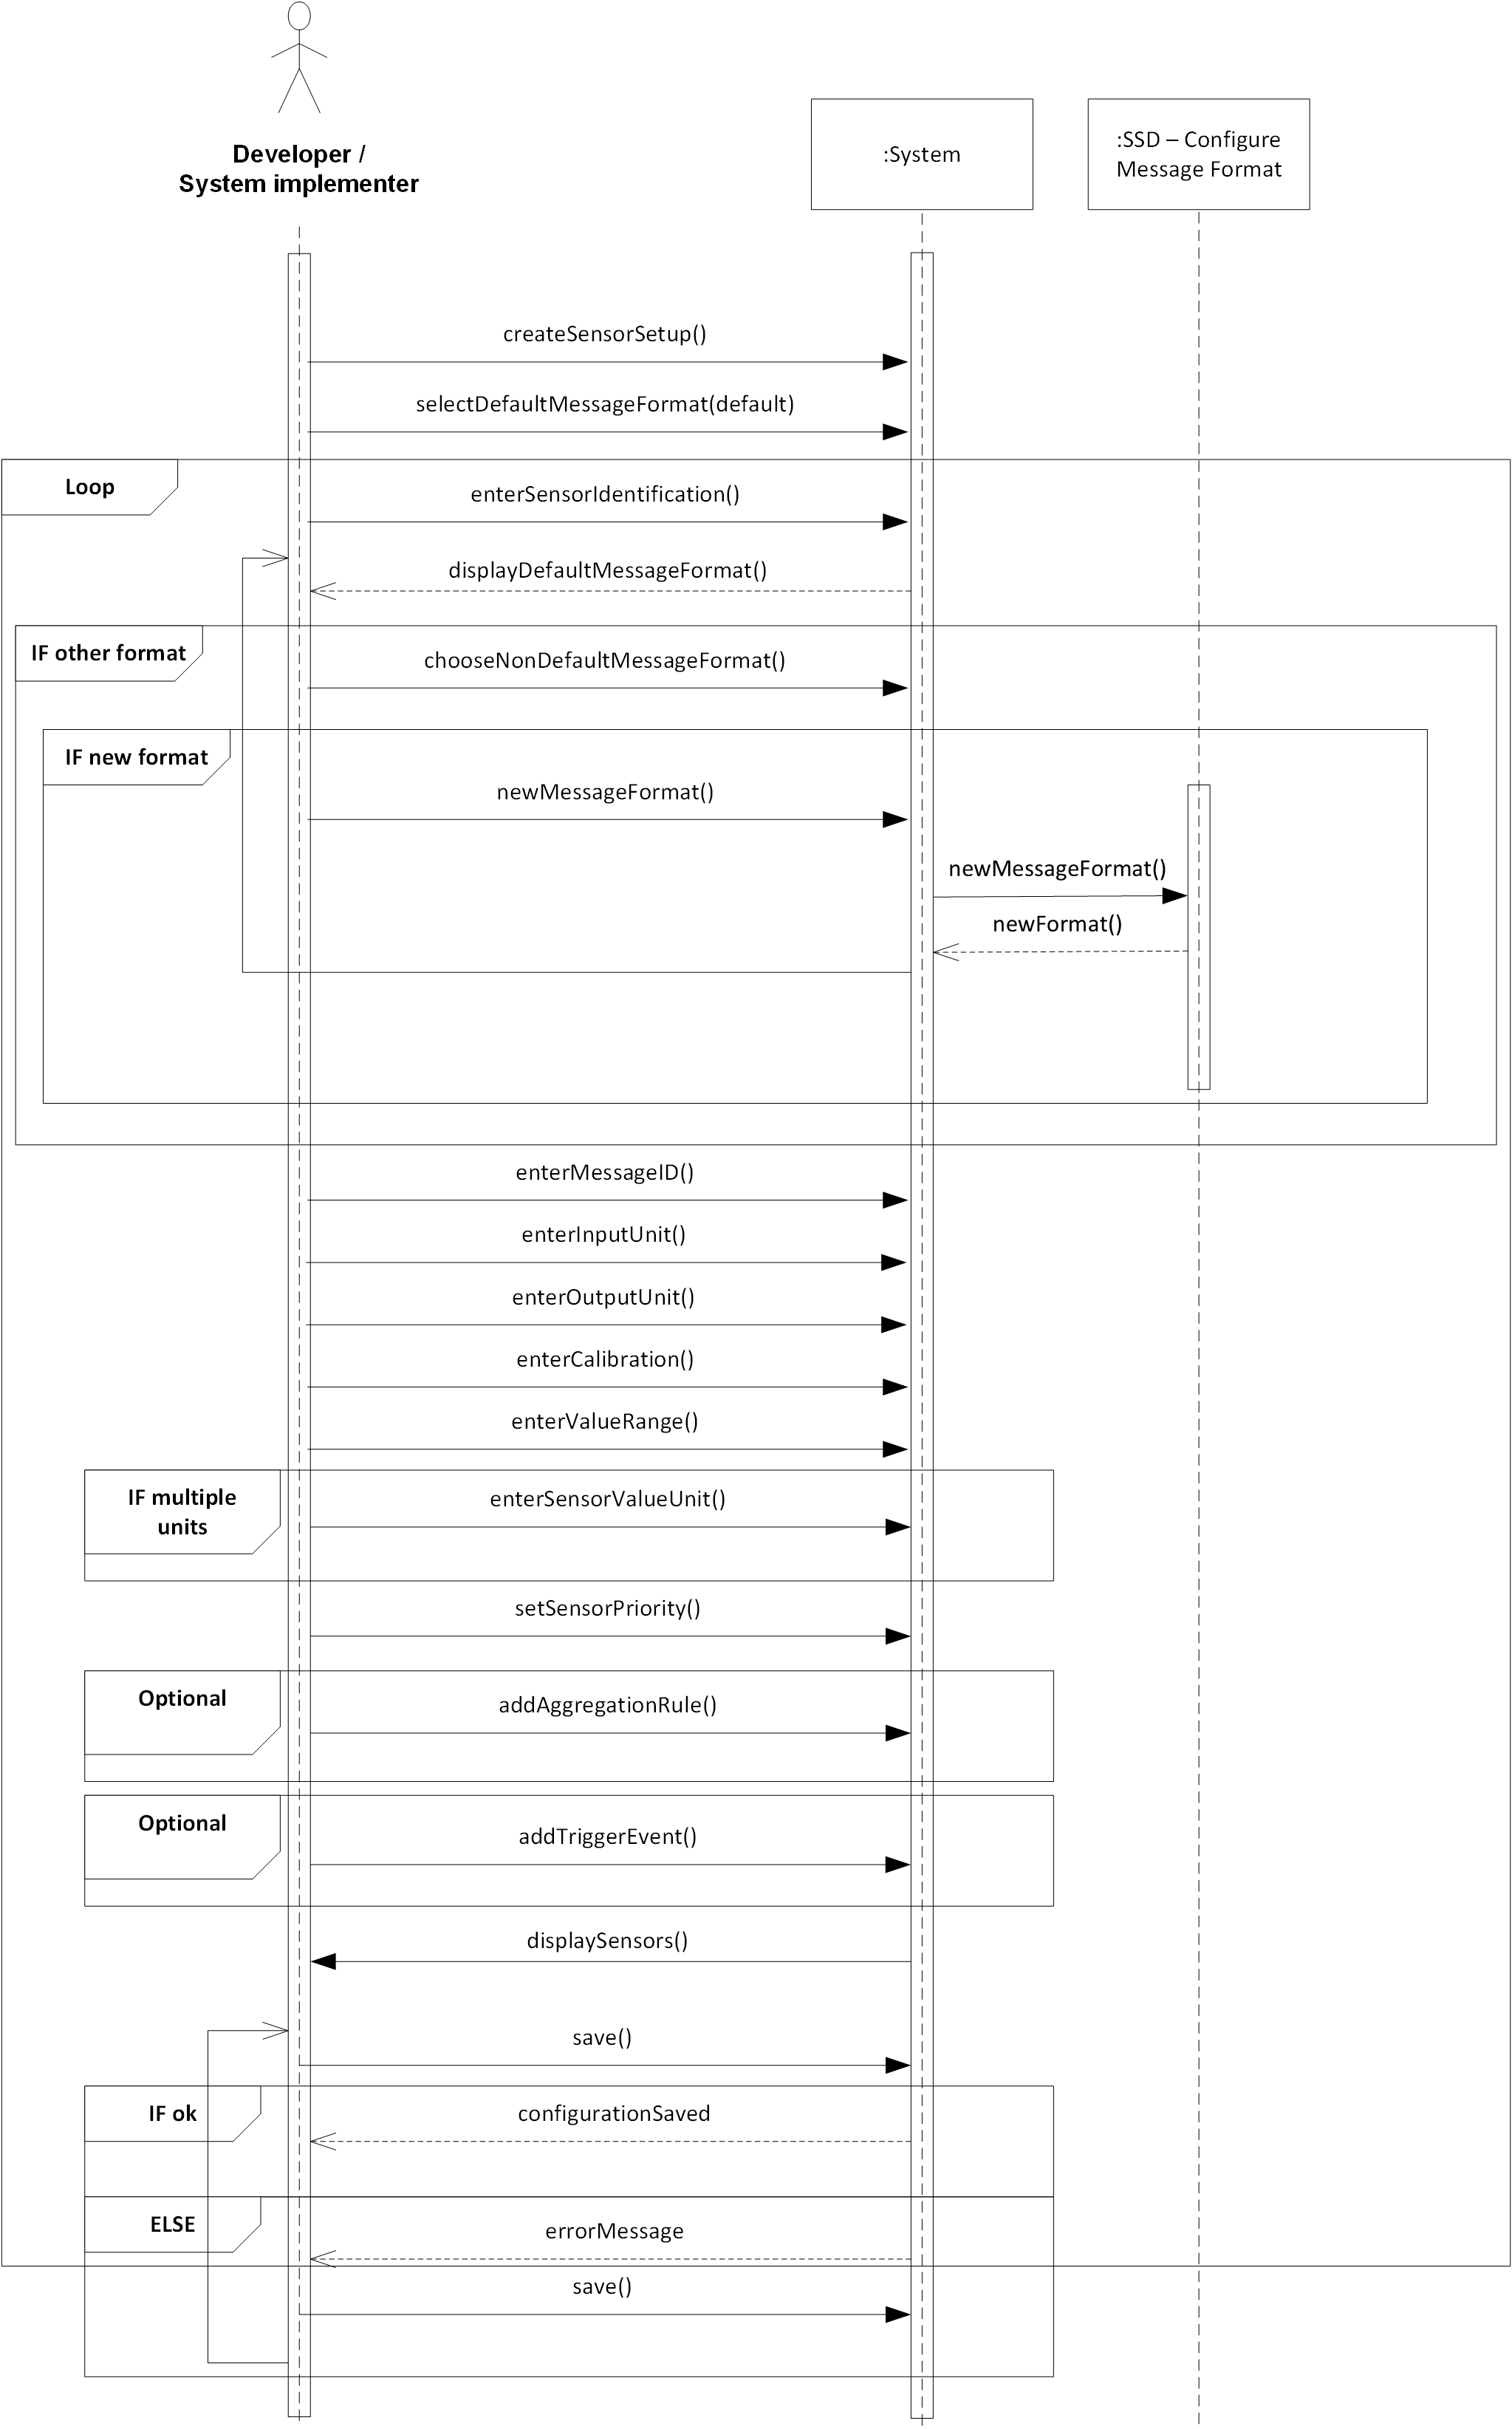
\includegraphics[height=0.9\textheight]{SSD-Configure-Sensors.png}
  \caption{SSD for UC\vref{uc_sensconf}}
  \label{fig:SSD-Configure-Sensors}
\end{figure}
\clearpage

\subsubsection{SSD - Configure Display}
\begin{figure}[!htbp]
  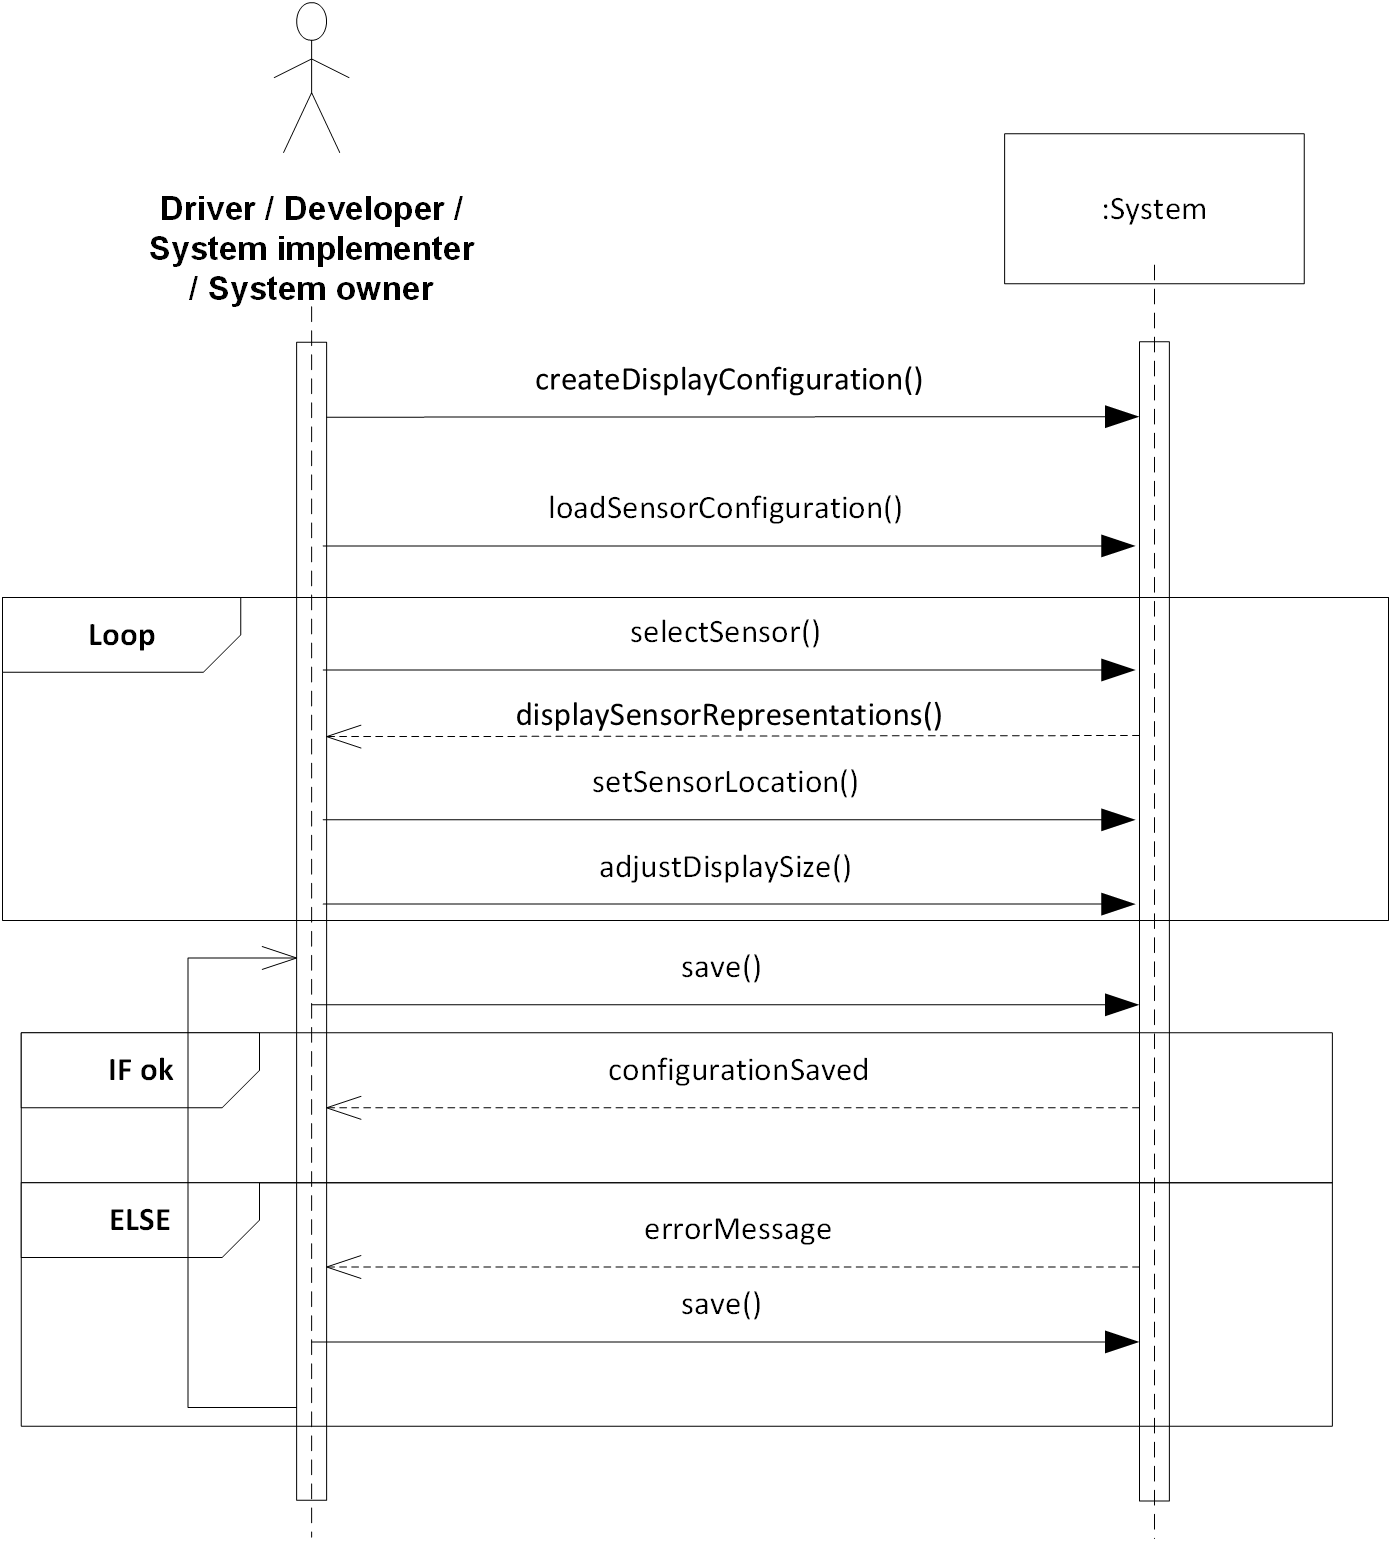
\includegraphics[width=\textwidth]{SSD-Configure-Display.png}
  \caption{SSD for UC\vref{uc_dispconf}}
  \label{fig:SSD-Configure-Display}
\end{figure}
\clearpage 


\subsubsection{SSD - Upload Configuration}
\begin{figure}[!htbp]
  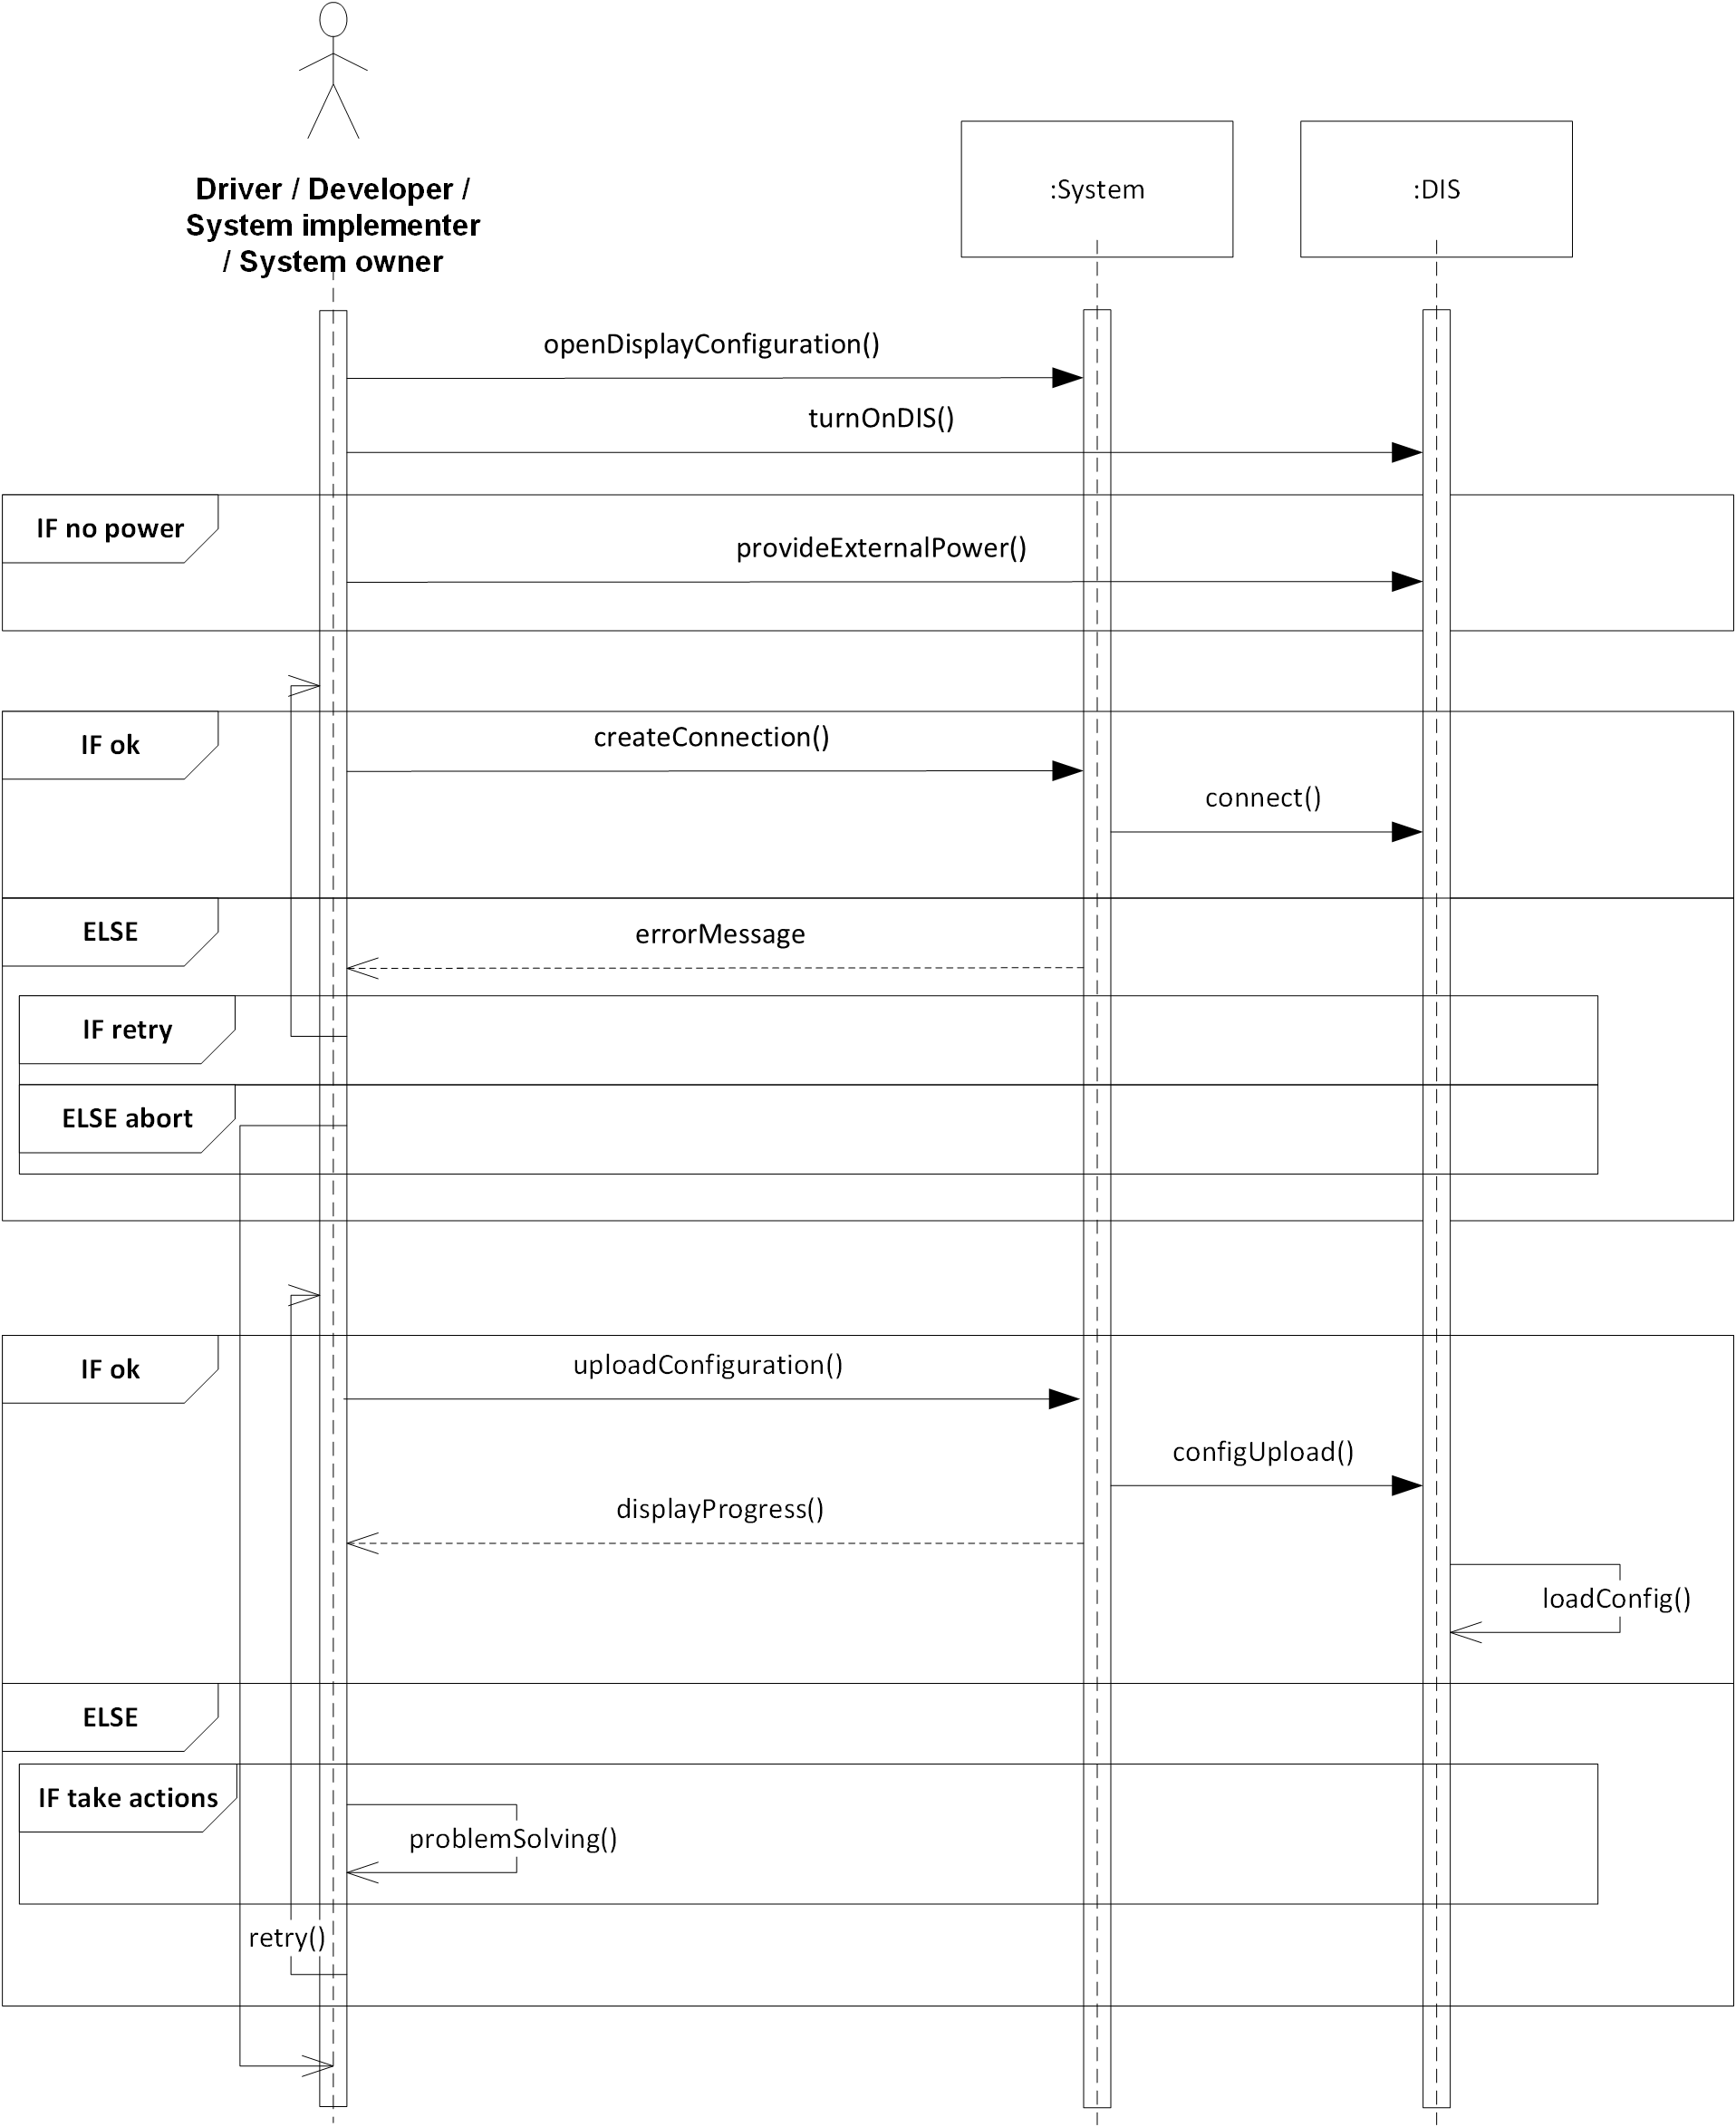
\includegraphics[width=\textwidth]{SSD-Upload-Configuration.png}
  \caption{SSD for UC\vref{uc_dispconf}}
  \label{fig:SSD-Upload-Configuration}
\end{figure}
\clearpage 


\subsubsection{SSD - Send message to driver}
\begin{figure}[!htbp]
  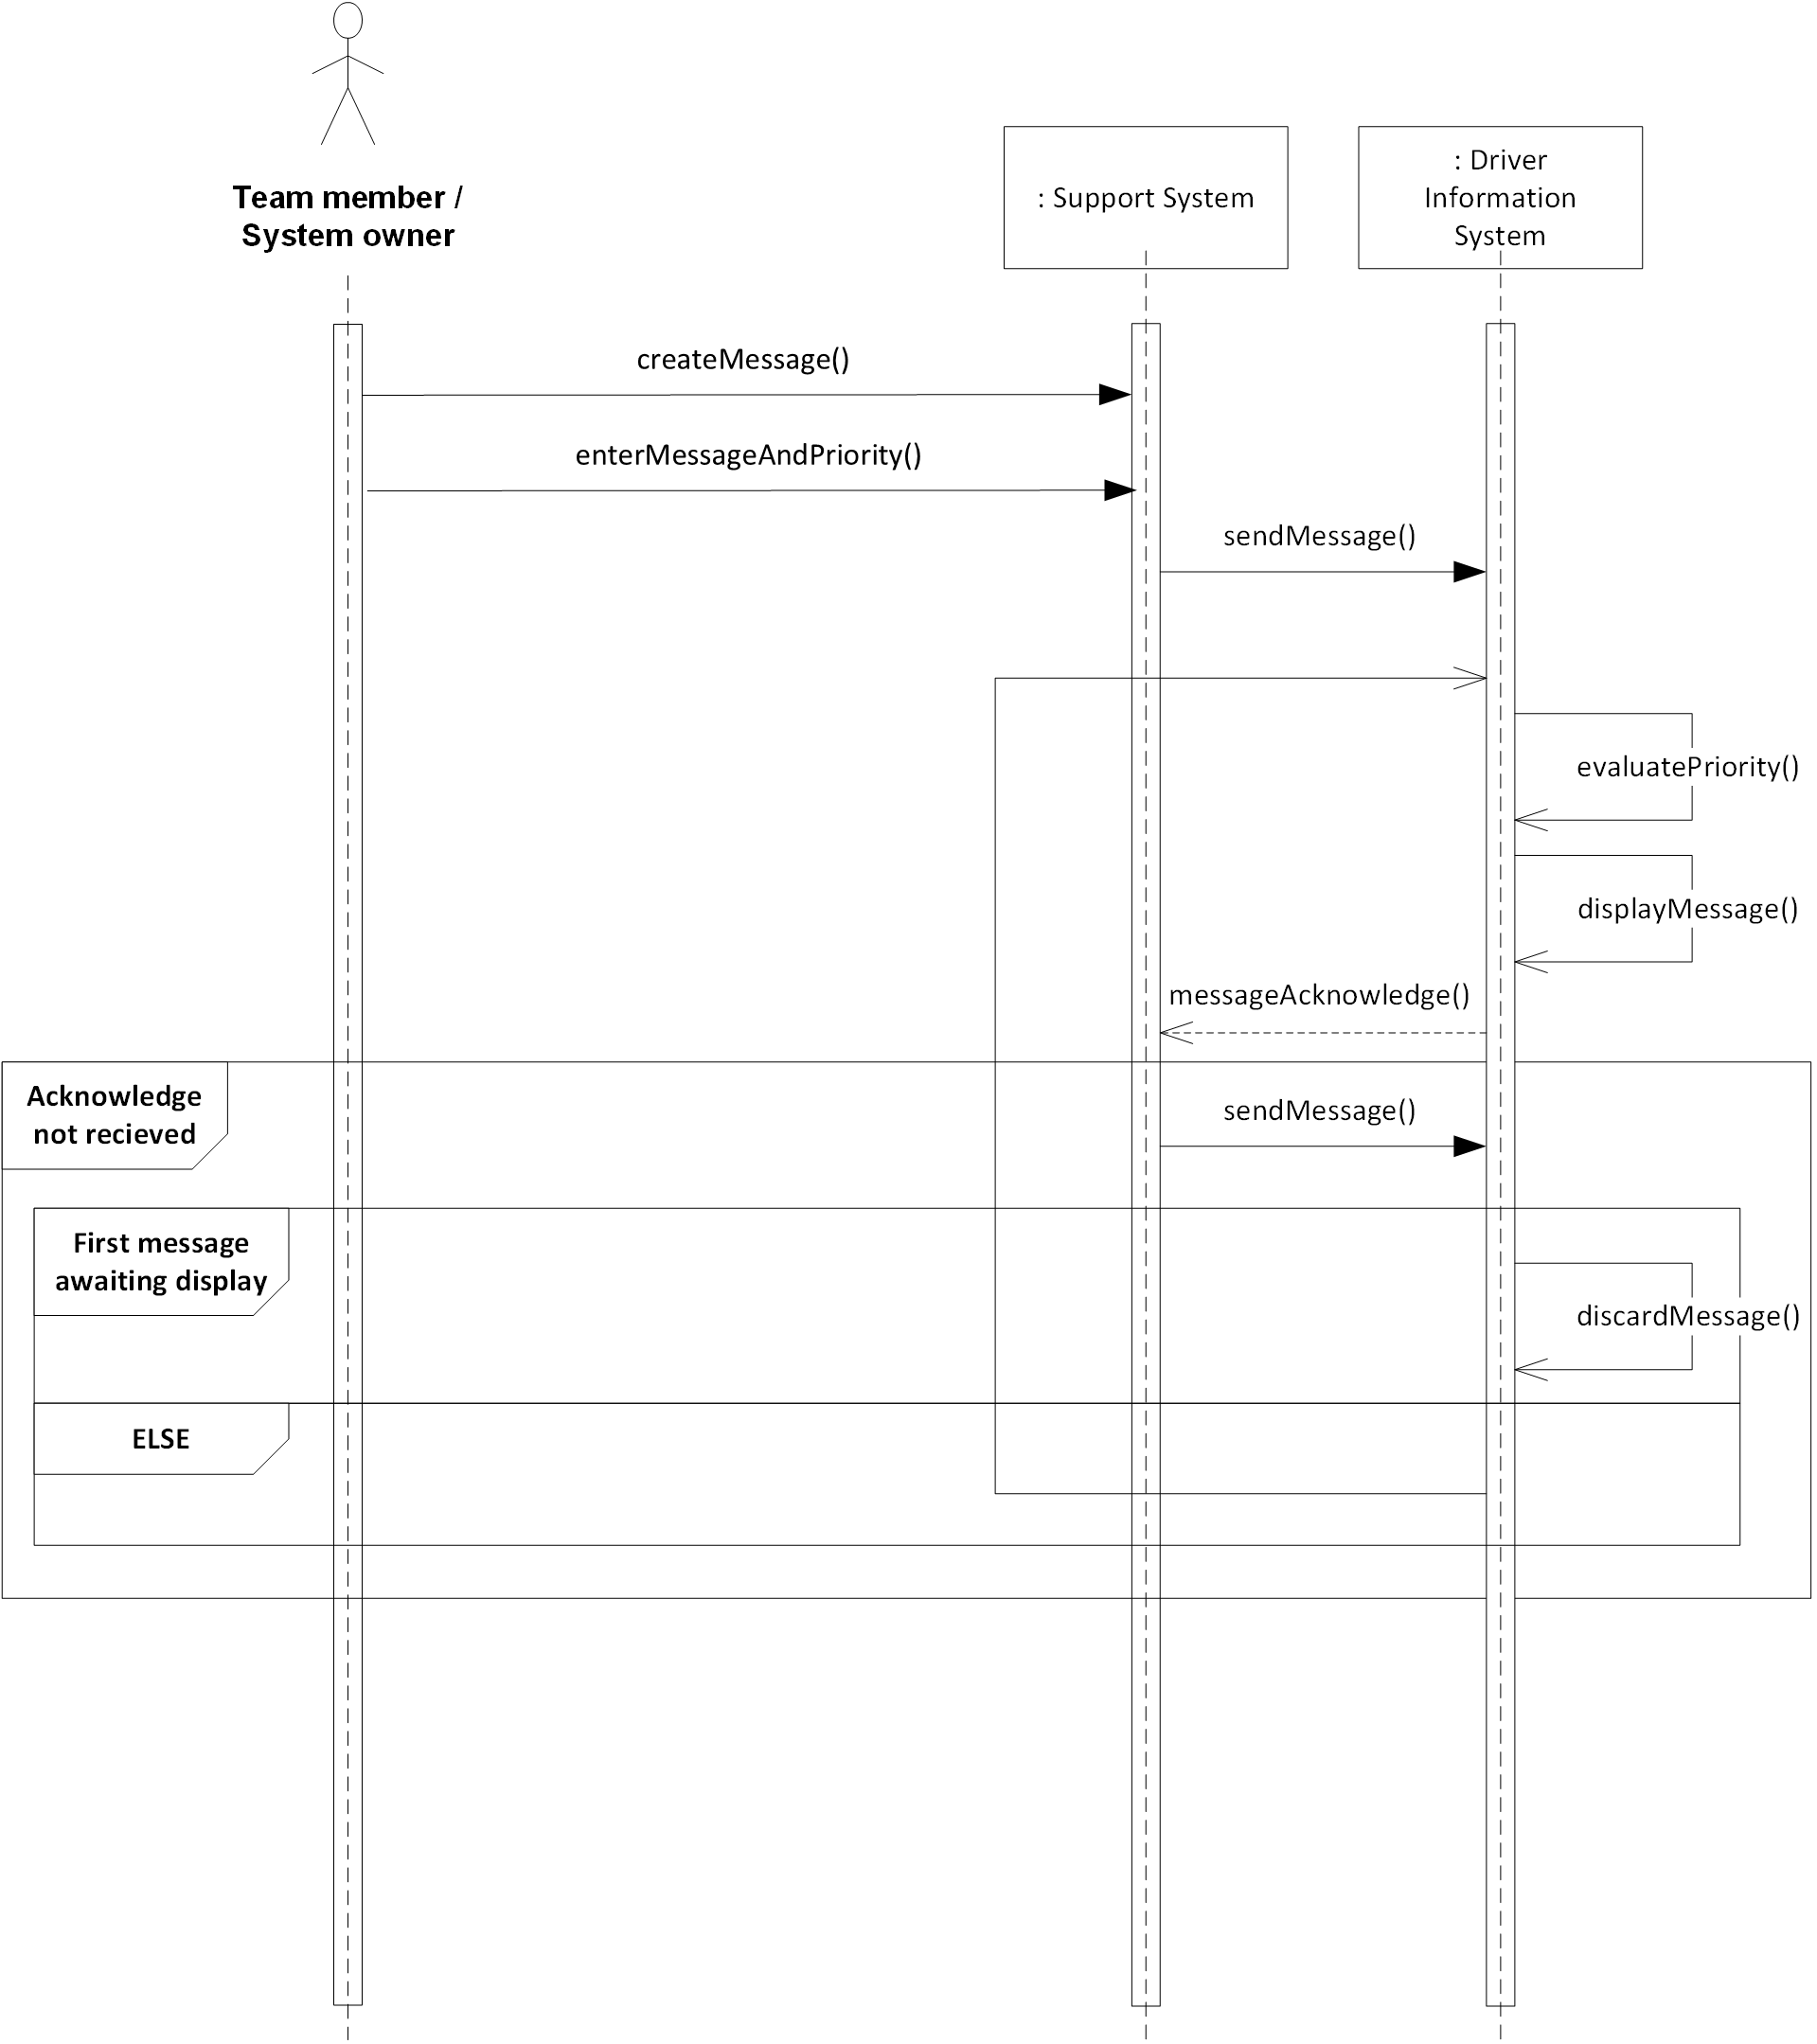
\includegraphics[width=\textwidth]{SSD-Send-Message.png}
  \caption{SSD for UC\vref{uc_dispconf}}
  \label{fig:SSD-Send-Message}
\end{figure}
\clearpage 


\subsubsection{SSD - Display Real Time Info}
\begin{figure}[!htbp]
  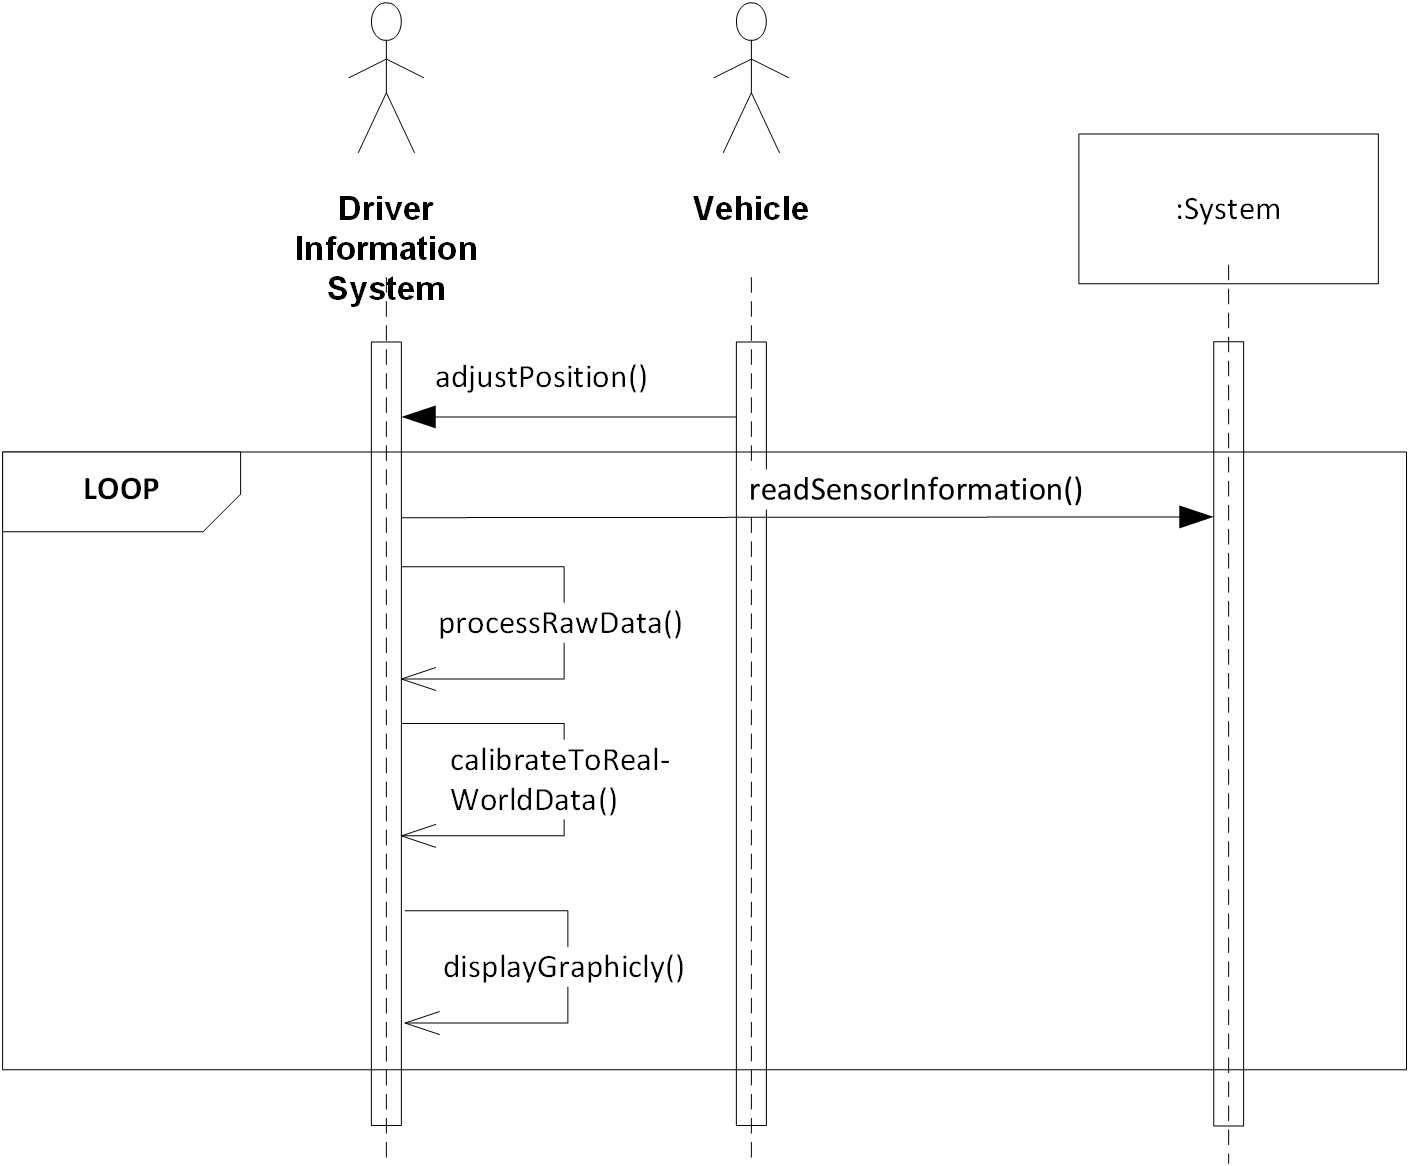
\includegraphics[width=\textwidth]{SSD-Display-Real-Time-Info.png}
  \caption{SSD for UC\vref{uc_dispconf}}
  \label{fig:SSD-Display-Real-Time-Info}
\end{figure}
\clearpage 


\section{Domain model}
\begin{figure}[!htbp]
  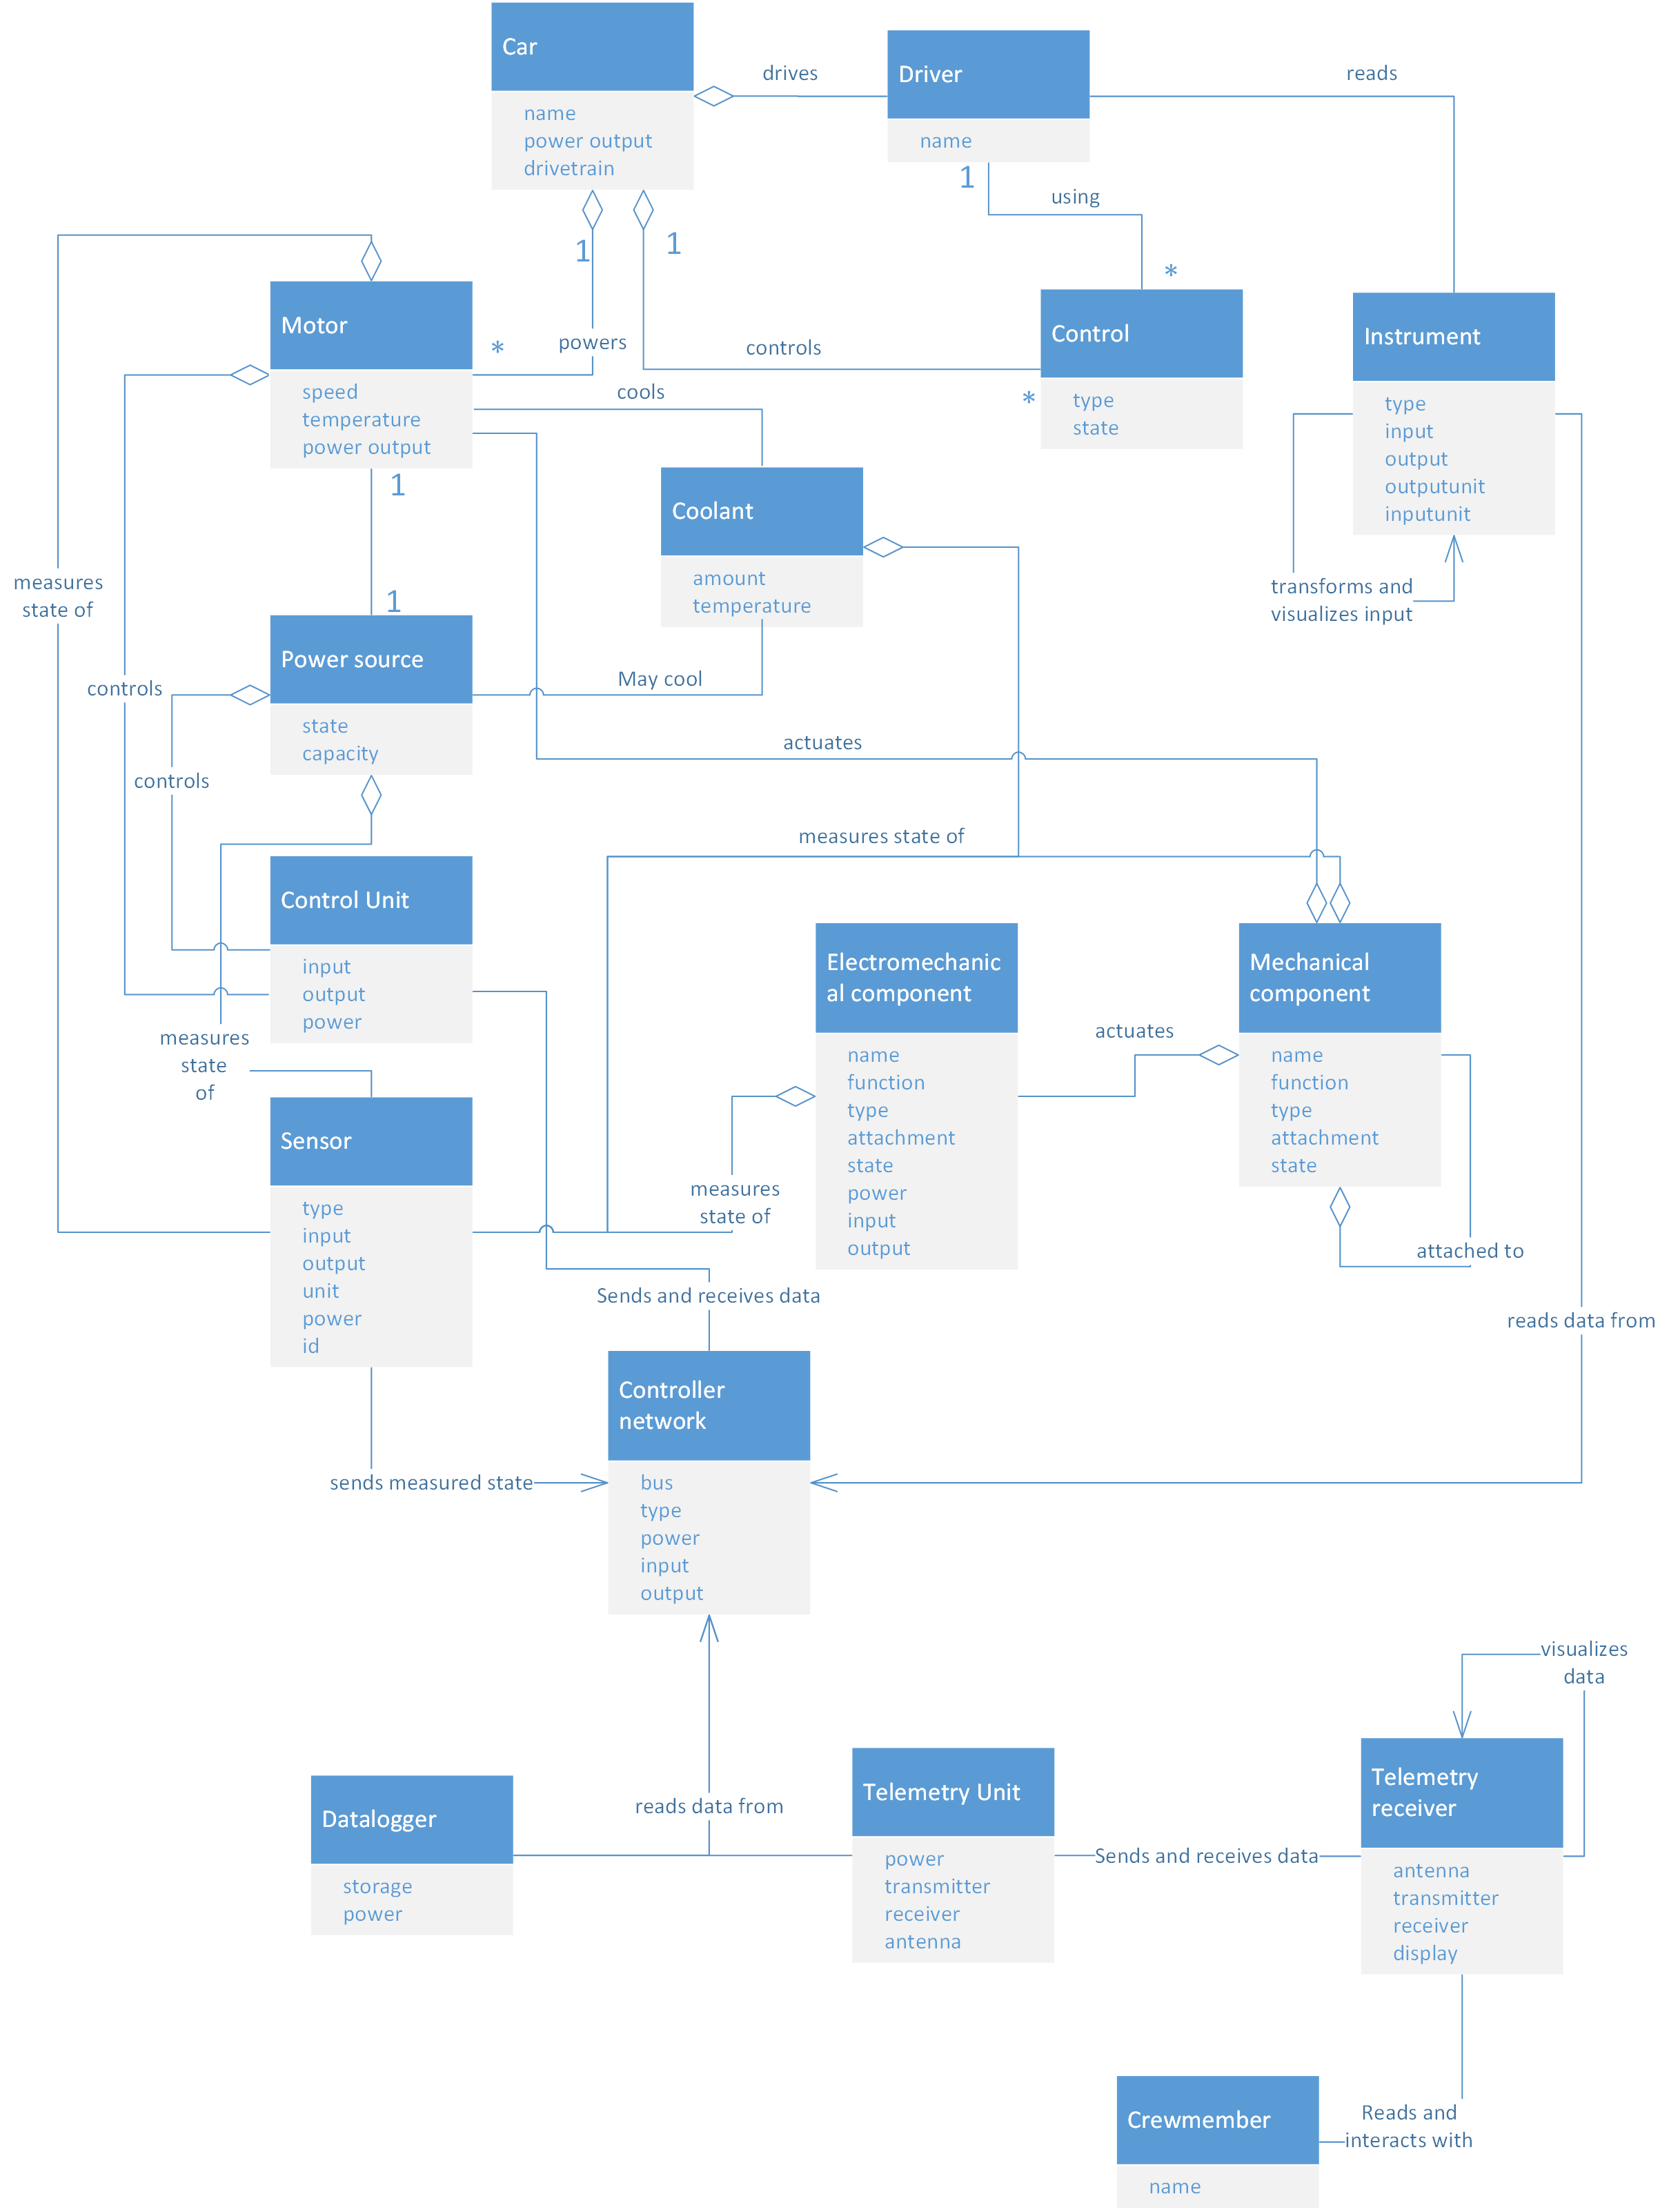
\includegraphics[width=\textwidth]{domain-model.png}
  %\caption{Model of }
  \label{fig:domain-model}
\end{figure}


\bibliography{../../bibliography}
\bibliographystyle{ieeetr}

\end{document}
